%% bare_conf.tex
%% V1.4b
%% 2015/08/26
%% by Michael Shell
%% See:
%% http://www.michaelshell.org/
%% for current contact information.
%%
%% This is a skeleton file demonstrating the use of IEEEtran.cls
%% (requires IEEEtran.cls version 1.8b or later) with an IEEE
%% conference paper.
%%
%% Support sites:
%% http://www.michaelshell.org/tex/ieeetran/
%% http://www.ctan.org/pkg/ieeetran
%% and
%% http://www.ieee.org/

%%*************************************************************************
%% Legal Notice:
%% This code is offered as-is without any warranty either expressed or
%% implied; without even the implied warranty of MERCHANTABILITY or
%% FITNESS FOR A PARTICULAR PURPOSE! 
%% User assumes all risk.
%% In no event shall the IEEE or any contributor to this code be liable for
%% any damages or losses, including, but not limited to, incidental,
%% consequential, or any other damages, resulting from the use or misuse
%% of any information contained here.
%%
%% All comments are the opinions of their respective authors and are not
%% necessarily endorsed by the IEEE.
%%
%% This work is distributed under the LaTeX Project Public License (LPPL)
%% ( http://www.latex-project.org/ ) version 1.3, and may be freely used,
%% distributed and modified. A copy of the LPPL, version 1.3, is included
%% in the base LaTeX documentation of all distributions of LaTeX released
%% 2003/12/01 or later.
%% Retain all contribution notices and credits.
%% ** Modified files should be clearly indicated as such, including  **
%% ** renaming them and changing author support contact information. **
%%*************************************************************************


% *** Authors should verify (and, if needed, correct) their LaTeX system  ***
% *** with the testflow diagnostic prior to trusting their LaTeX platform ***
% *** with production work. The IEEE's font choices and paper sizes can   ***
% *** trigger bugs that do not appear when using other class files.       ***                          ***
% The testflow support page is at:
% http://www.michaelshell.org/tex/testflow/



\documentclass[conference]{IEEEtran}
% Some Computer Society conferences also require the compsoc mode option,
% but others use the standard conference format.
%
% If IEEEtran.cls has not been installed into the LaTeX system files,
% manually specify the path to it like:
% \documentclass[conference]{../sty/IEEEtran}





% Some very useful LaTeX packages include:
% (uncomment the ones you want to load)


% *** MISC UTILITY PACKAGES ***
%
%\usepackage{ifpdf}
% Heiko Oberdiek's ifpdf.sty is very useful if you need conditional
% compilation based on whether the output is pdf or dvi.
% usage:
% \ifpdf
%   % pdf code
% \else
%   % dvi code
% \fi
% The latest version of ifpdf.sty can be obtained from:
% http://www.ctan.org/pkg/ifpdf
% Also, note that IEEEtran.cls V1.7 and later provides a builtin
% \ifCLASSINFOpdf conditional that works the same way.
% When switching from latex to pdflatex and vice-versa, the compiler may
% have to be run twice to clear warning/error messages.


\usepackage{hyperref}




% *** CITATION PACKAGES ***
%
\usepackage{cite}
% cite.sty was written by Donald Arseneau
% V1.6 and later of IEEEtran pre-defines the format of the cite.sty package
% \cite{} output to follow that of the IEEE. Loading the cite package will
% result in citation numbers being automatically sorted and properly
% "compressed/ranged". e.g., [1], [9], [2], [7], [5], [6] without using
% cite.sty will become [1], [2], [5]--[7], [9] using cite.sty. cite.sty's
% \cite will automatically add leading space, if needed. Use cite.sty's
% noadjust option (cite.sty V3.8 and later) if you want to turn this off
% such as if a citation ever needs to be enclosed in parenthesis.
% cite.sty is already installed on most LaTeX systems. Be sure and use
% version 5.0 (2009-03-20) and later if using hyperref.sty.
% The latest version can be obtained at:
% http://www.ctan.org/pkg/cite
% The documentation is contained in the cite.sty file itself.






% *** GRAPHICS RELATED PACKAGES ***
%
\ifCLASSINFOpdf
  % \usepackage[pdftex]{graphicx}
  % declare the path(s) where your graphic files are
  % \graphicspath{{../pdf/}{../jpeg/}}
  % and their extensions so you won't have to specify these with
  % every instance of \includegraphics
  % \DeclareGraphicsExtensions{.pdf,.jpeg,.png}
\else
  % or other class option (dvipsone, dvipdf, if not using dvips). graphicx
  % will default to the driver specified in the system graphics.cfg if no
  % driver is specified.
  % \usepackage[dvips]{graphicx}
  % declare the path(s) where your graphic files are
  % \graphicspath{{../eps/}}
  % and their extensions so you won't have to specify these with
  % every instance of \includegraphics
  % \DeclareGraphicsExtensions{.eps}
\fi
% graphicx was written by David Carlisle and Sebastian Rahtz. It is
% required if you want graphics, photos, etc. graphicx.sty is already
% installed on most LaTeX systems. The latest version and documentation
% can be obtained at: 
% http://www.ctan.org/pkg/graphicx
% Another good source of documentation is "Using Imported Graphics in
% LaTeX2e" by Keith Reckdahl which can be found at:
% http://www.ctan.org/pkg/epslatex
%
% latex, and pdflatex in dvi mode, support graphics in encapsulated
% postscript (.eps) format. pdflatex in pdf mode supports graphics
% in .pdf, .jpeg, .png and .mps (metapost) formats. Users should ensure
% that all non-photo figures use a vector format (.eps, .pdf, .mps) and
% not a bitmapped formats (.jpeg, .png). The IEEE frowns on bitmapped formats
% which can result in "jaggedy"/blurry rendering of lines and letters as
% well as large increases in file sizes.
%
% You can find documentation about the pdfTeX application at:
% http://www.tug.org/applications/pdftex





% *** MATH PACKAGES ***
%
%\usepackage{amsmath}
% A popular package from the American Mathematical Society that provides
% many useful and powerful commands for dealing with mathematics.
%
% Note that the amsmath package sets \interdisplaylinepenalty to 10000
% thus preventing page breaks from occurring within multiline equations. Use:
%\interdisplaylinepenalty=2500
% after loading amsmath to restore such page breaks as IEEEtran.cls normally
% does. amsmath.sty is already installed on most LaTeX systems. The latest
% version and documentation can be obtained at:
% http://www.ctan.org/pkg/amsmath


\usepackage{fancyhdr}
\pagestyle{fancy}
\fancyhf{} % clear all header and footer fields
\fancyfoot[R]{\thepage} % Page number on the right footer






% *** SPECIALIZED LIST PACKAGES ***
%
%\usepackage{algorithmic}
% algorithmic.sty was written by Peter Williams and Rogerio Brito.
% This package provides an algorithmic environment fo describing algorithms.
% You can use the algorithmic environment in-text or within a figure
% environment to provide for a floating algorithm. Do NOT use the algorithm
% floating environment provided by algorithm.sty (by the same authors) or
% algorithm2e.sty (by Christophe Fiorio) as the IEEE does not use dedicated
% algorithm float types and packages that provide these will not provide
% correct IEEE style captions. The latest version and documentation of
% algorithmic.sty can be obtained at:
% http://www.ctan.org/pkg/algorithms
% Also of interest may be the (relatively newer and more customizable)
% algorithmicx.sty package by Szasz Janos:
% http://www.ctan.org/pkg/algorithmicx




% *** ALIGNMENT PACKAGES ***
%
%\usepackage{array}
% Frank Mittelbach's and David Carlisle's array.sty patches and improves
% the standard LaTeX2e array and tabular environments to provide better
% appearance and additional user controls. As the default LaTeX2e table
% generation code is lacking to the point of almost being broken with
% respect to the quality of the end results, all users are strongly
% advised to use an enhanced (at the very least that provided by array.sty)
% set of table tools. array.sty is already installed on most systems. The
% latest version and documentation can be obtained at:
% http://www.ctan.org/pkg/array


% IEEEtran contains the IEEEeqnarray family of commands that can be used to
% generate multiline equations as well as matrices, tables, etc., of high
% quality.




% *** SUBFIGURE PACKAGES ***
%\ifCLASSOPTIONcompsoc
%  \usepackage[caption=false,font=normalsize,labelfont=sf,textfont=sf]{subfig}
%\else
%  \usepackage[caption=false,font=footnotesize]{subfig}
%\fi
% subfig.sty, written by Steven Douglas Cochran, is the modern replacement
% for subfigure.sty, the latter of which is no longer maintained and is
% incompatible with some LaTeX packages including fixltx2e. However,
% subfig.sty requires and automatically loads Axel Sommerfeldt's caption.sty
% which will override IEEEtran.cls' handling of captions and this will result
% in non-IEEE style figure/table captions. To prevent this problem, be sure
% and invoke subfig.sty's "caption=false" package option (available since
% subfig.sty version 1.3, 2005/06/28) as this is will preserve IEEEtran.cls
% handling of captions.
% Note that the Computer Society format requires a larger sans serif font
% than the serif footnote size font used in traditional IEEE formatting
% and thus the need to invoke different subfig.sty package options depending
% on whether compsoc mode has been enabled.
%
% The latest version and documentation of subfig.sty can be obtained at:
% http://www.ctan.org/pkg/subfig




% *** FLOAT PACKAGES ***
%
%\usepackage{fixltx2e}
% fixltx2e, the successor to the earlier fix2col.sty, was written by
% Frank Mittelbach and David Carlisle. This package corrects a few problems
% in the LaTeX2e kernel, the most notable of which is that in current
% LaTeX2e releases, the ordering of single and double column floats is not
% guaranteed to be preserved. Thus, an unpatched LaTeX2e can allow a
% single column figure to be placed prior to an earlier double column
% figure.
% Be aware that LaTeX2e kernels dated 2015 and later have fixltx2e.sty's
% corrections already built into the system in which case a warning will
% be issued if an attempt is made to load fixltx2e.sty as it is no longer
% needed.
% The latest version and documentation can be found at:
% http://www.ctan.org/pkg/fixltx2e


%\usepackage{stfloats}
% stfloats.sty was written by Sigitas Tolusis. This package gives LaTeX2e
% the ability to do double column floats at the bottom of the page as well
% as the top. (e.g., "\begin{figure*}[!b]" is not normally possible in
% LaTeX2e). It also provides a command:
%\fnbelowfloat
% to enable the placement of footnotes below bottom floats (the standard
% LaTeX2e kernel puts them above bottom floats). This is an invasive package
% which rewrites many portions of the LaTeX2e float routines. It may not work
% with other packages that modify the LaTeX2e float routines. The latest
% version and documentation can be obtained at:
% http://www.ctan.org/pkg/stfloats
% Do not use the stfloats baselinefloat ability as the IEEE does not allow
% \baselineskip to stretch. Authors submitting work to the IEEE should note
% that the IEEE rarely uses double column equations and that authors should try
% to avoid such use. Do not be tempted to use the cuted.sty or midfloat.sty
% packages (also by Sigitas Tolusis) as the IEEE does not format its papers in
% such ways.
% Do not attempt to use stfloats with fixltx2e as they are incompatible.
% Instead, use Morten Hogholm'a dblfloatfix which combines the features
% of both fixltx2e and stfloats:
%
% \usepackage{dblfloatfix}
% The latest version can be found at:
% http://www.ctan.org/pkg/dblfloatfix




% *** PDF, URL AND HYPERLINK PACKAGES ***
%
\usepackage{url}
% url.sty was written by Donald Arseneau. It provides better support for
% handling and breaking URLs. url.sty is already installed on most LaTeX
% systems. The latest version and documentation can be obtained at:
% http://www.ctan.org/pkg/url
% Basically, \url{my_url_here}.


\usepackage{graphicx}

% *** Do not adjust lengths that control margins, column widths, etc. ***
% *** Do not use packages that alter fonts (such as pslatex).         ***
% There should be no need to do such things with IEEEtran.cls V1.6 and later.
% (Unless specifically asked to do so by the journal or conference you plan
% to submit to, of course. )


% correct bad hyphenation here
\hyphenation{op-tical net-works semi-conduc-tor}


\begin{document}
%
% paper title
% Titles are generally capitalized except for words such as a, an, and, as,
% at, but, by, for, in, nor, of, on, or, the, to and up, which are usually
% not capitalized unless they are the first or last word of the title.
% Linebreaks \\ can be used within to get better formatting as desired.
% Do not put math or special symbols in the title.
\title{Soft IP-Cores: RISC-V Processors and more}


% author names and affiliations
% use a multiple column layout for up to three different
% affiliations
\author{\IEEEauthorblockN{Doluwamu Taiwo Kuye}
\IEEEauthorblockA{Hamm-Lippstadt University of Applied Sciences\\
Email: Doluwamu-Taiwo.kuye@stud.hshl.de}}




% conference papers do not typically use \thanks and this command
% is locked out in conference mode. If really needed, such as for
% the acknowledgment of grants, issue a \IEEEoverridecommandlockouts
% after \documentclass

% for over three affiliations, or if they all won't fit within the width
% of the page, use this alternative format:
% 
%\author{\IEEEauthorblockN{Michael Shell\IEEEauthorrefmark{1},
%Homer Simpson\IEEEauthorrefmark{2},
%James Kirk\IEEEauthorrefmark{3}, 
%Montgomery Scott\IEEEauthorrefmark{3} and
%Eldon Tyrell\IEEEauthorrefmark{4}}
%\IEEEauthorblockA{\IEEEauthorrefmark{1}School of Electrical and Computer Engineering\\
%Georgia Institute of Technology,
%Atlanta, Georgia 30332--0250\\ Email: see http://www.michaelshell.org/contact.html}
%\IEEEauthorblockA{\IEEEauthorrefmark{2}Twentieth Century Fox, Springfield, USA\\
%Email: homer@thesimpsons.com}
%\IEEEauthorblockA{\IEEEauthorrefmark{3}Starfleet Academy, San Francisco, California 96678-2391\\
%Telephone: (800) 555--1212, Fax: (888) 555--1212}
%\IEEEauthorblockA{\IEEEauthorrefmark{4}Tyrell Inc., 123 Replicant Street, Los Angeles, California 90210--4321}}




% use for special paper notices
%\IEEEspecialpapernotice{(Invited Paper)}




% make the title area
\maketitle

% As a general rule, do not put math, special symbols or citations
% in the abstract
\begin{abstract}
In this study, we explore the dynamic field of soft IP-cores, with a particular focus on RISC-V processors. Our analysis begins with a distinction between soft and hardcore processors, underscoring the advantages of softcores, notably their flexibility and customizability. We delve deep into the RISC-V architecture, an open-source initiative that stands out for its adaptability and wide-ranging applicability. Through a comparative examination of various soft RISC-V cores, we present their suitability for diverse applications. Additionally, we address the challenges inherent in soft-core processors, such as vulnerability to Single Event Upsets (SEUs), performance limitations, and scalability issues, and discuss their implementation in real-world scenarios. This study aims to provide a comprehensive understanding of the current state of soft IP-cores, particularly RISC-V processors, and their significant role in the landscape of Integrated Circuit (IC) design.
\end{abstract}

% no keywords




% For peer review papers, you can put extra information on the cover
% page as needed:
% \ifCLASSOPTIONpeerreview
% \begin{center} \bfseries EDICS Category: 3-BBND \end{center}
% \fi
%
% For peerreview papers, this IEEEtran command inserts a page break and
% creates the second title. It will be ignored for other modes.
\IEEEpeerreviewmaketitle



\section{Background}
Hardcore processors have long been dominant in the field of IC design and system-on-chip devices. These processors, physically constructed on silicon at the transistor level, provided a specialized and efficient solution \cite{1}. However, the emergence of challenges related to configurability, customization, and prototyping inefficiencies has prompted a notable shift in the design landscape.

\begin{figure}[ht]
\begin{center}
  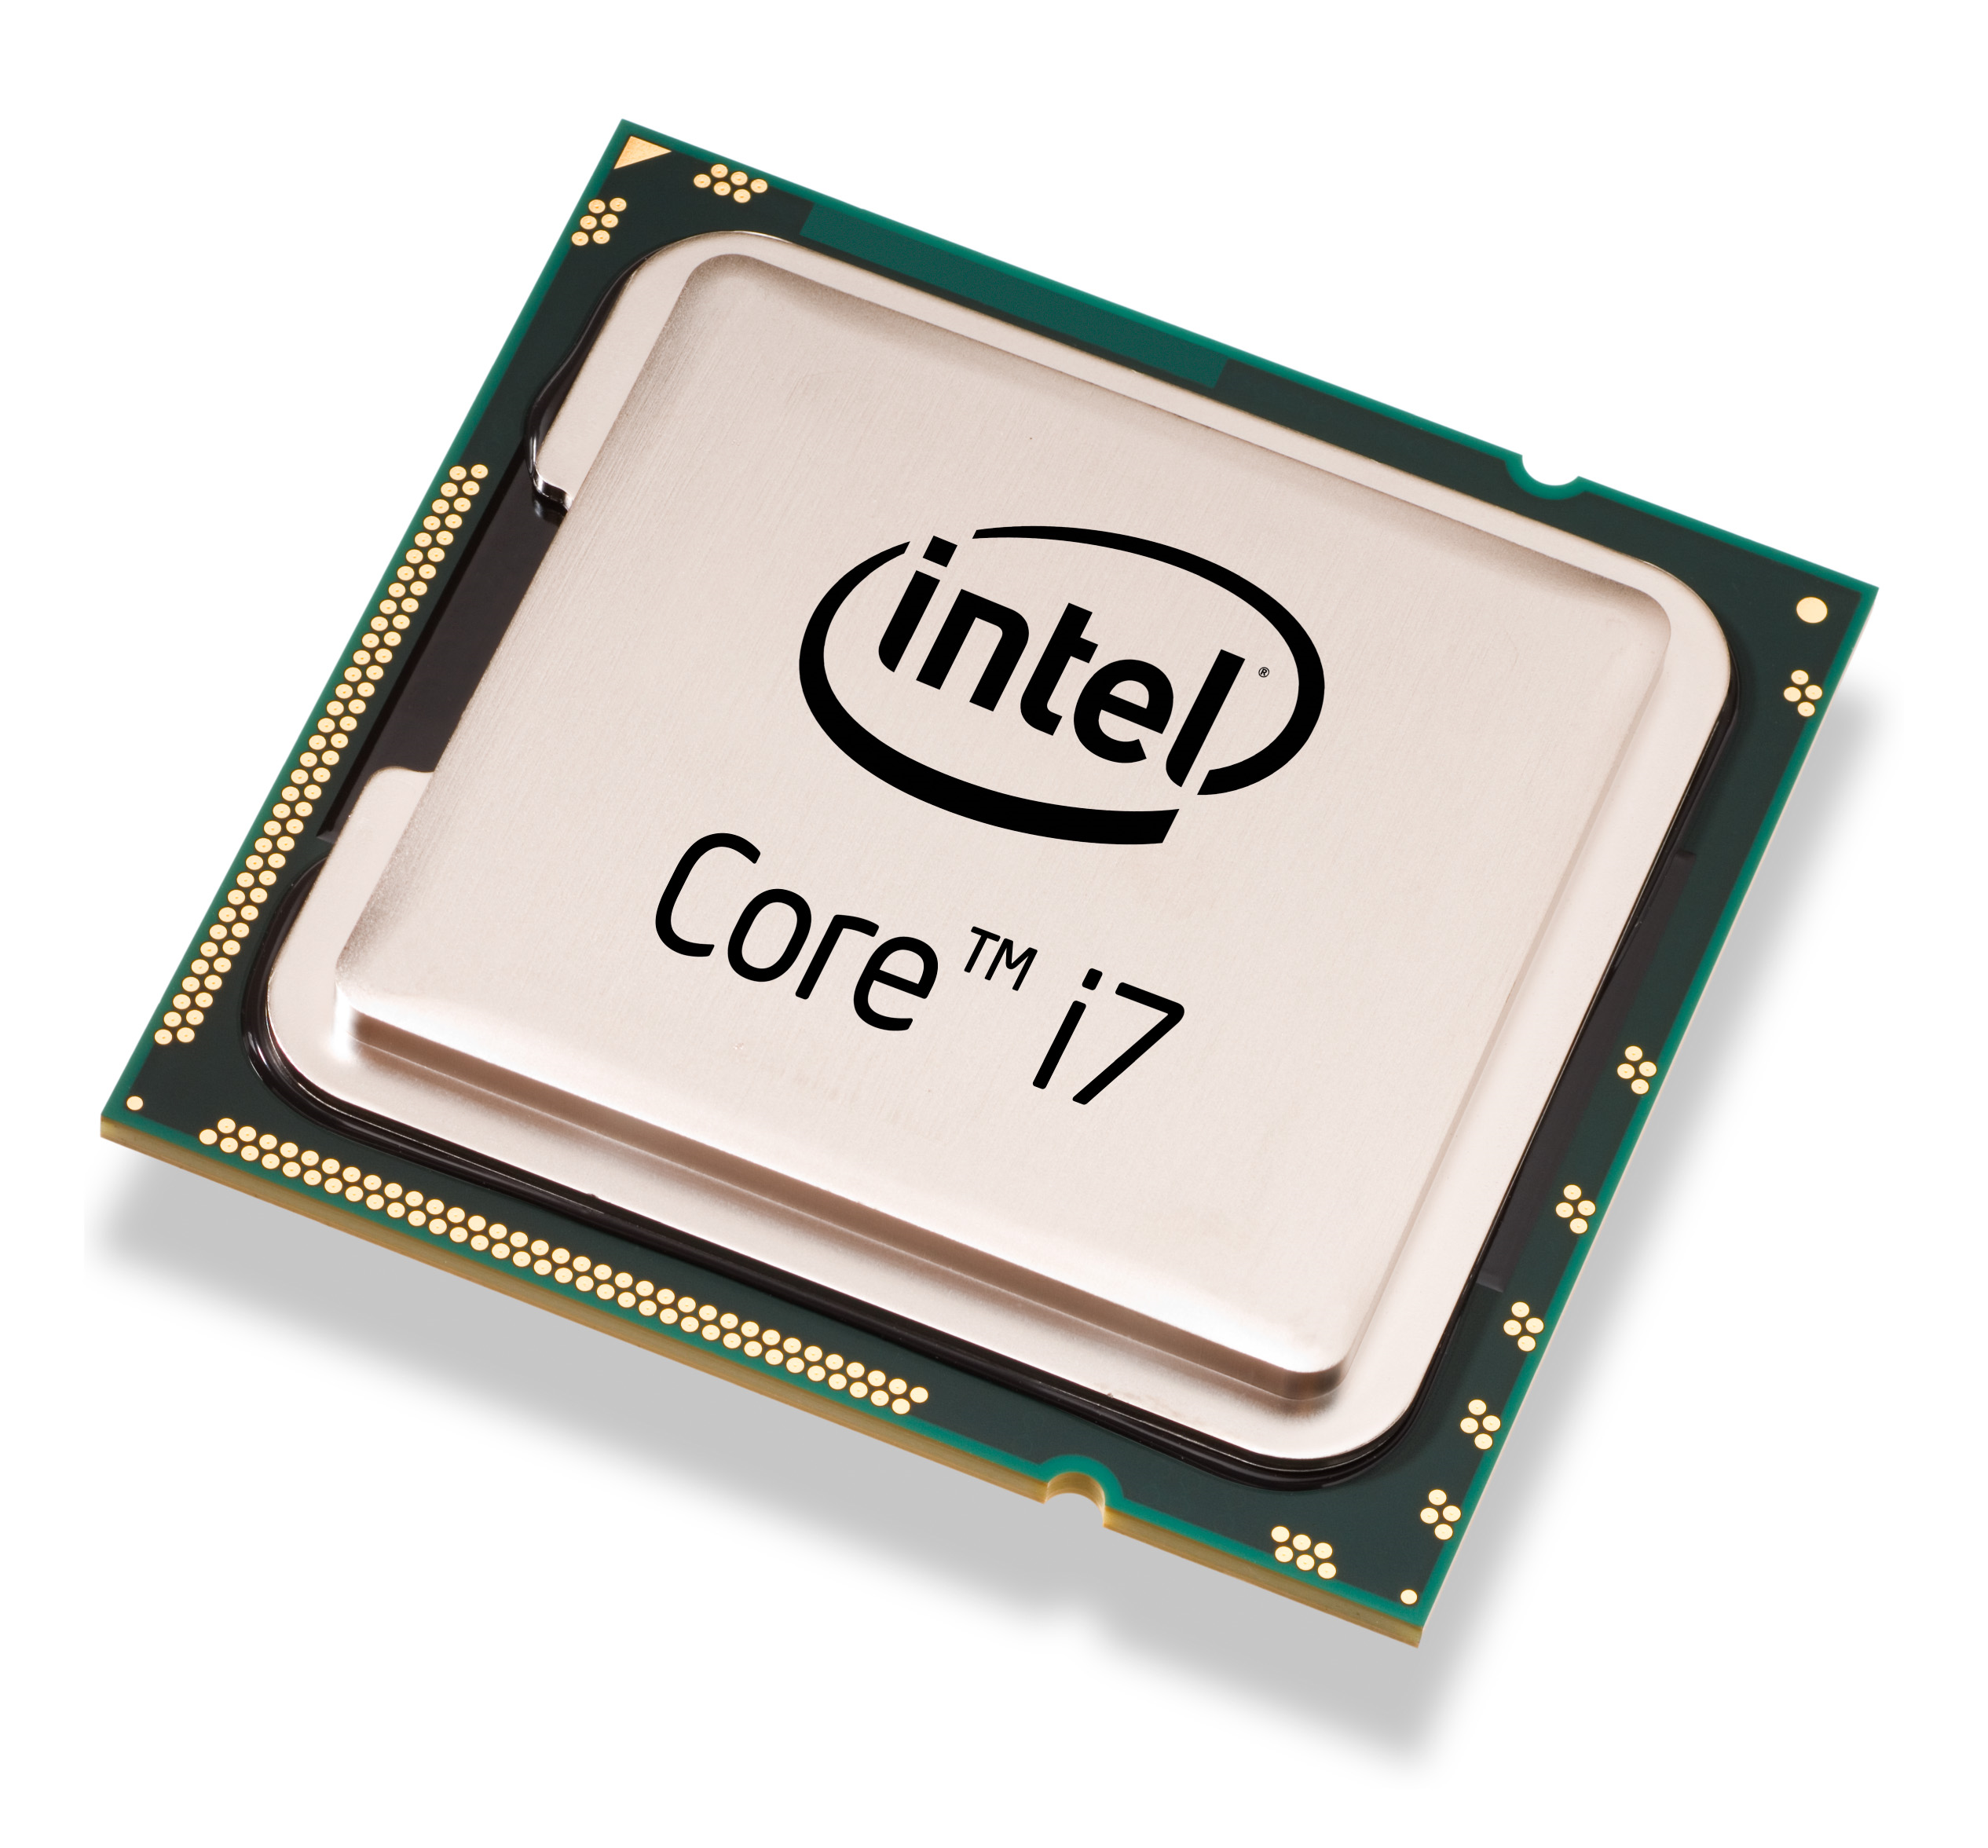
\includegraphics[scale=0.25]{download37 (1).png}
\end{center}
  \caption{Intel i7 Hardcore processor}
  \label{fig:1}
\end{figure}
This resulted in the development of soft processors. Softcore processors have a critical advantage, which is configurability. This means they can be tailored to specific application needs, optimising performance and power usage. This innovative flexibility addresses the limitations of fixed architectures in hardcore processors and also provides added advantages like rapid prototyping.
In the contemporary sphere of IC design, soft cores have become indispensable. They effectively navigate challenges and provide a dynamic solution to meet the ever-evolving demands of the field \cite{1}.

\begin{figure}[ht]
\begin{center}
  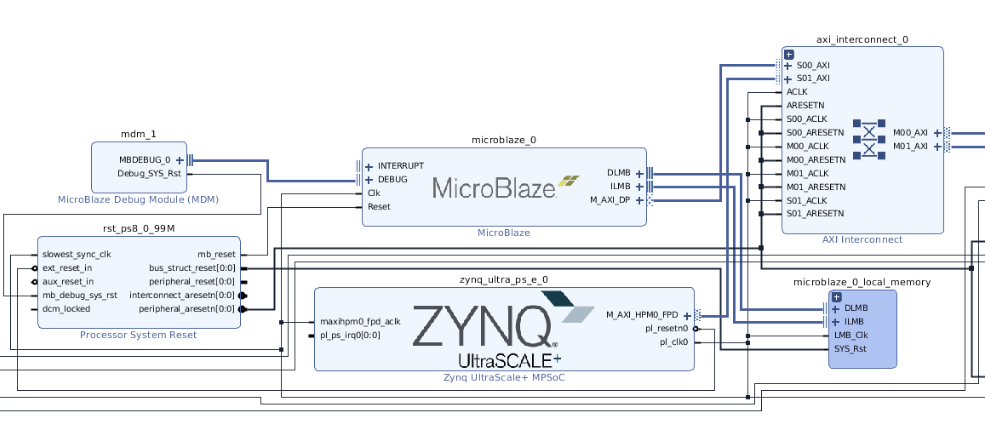
\includegraphics[scale=0.28]{Screenshot 2023-11-01 at 13.41.08 (1).png}
\end{center}
  \caption{Microblaze Softcore -In Vivado design Environment}
  \label{fig:2}
\end{figure}

\subsection{Significance of Soft IP-Cores in IC Design}
The evolution of soft processors in integrated circuit (IC) design has been propelled by a dynamic interplay of challenges faced by hardware architects. Traditional ASIC designs grapple with intricacies such as power consumption, compactness, and signal integrity, demanding a departure from the rigidity of microprocessors. The accelerated obsolescence of microcontrollers further intensifies the need for adaptable solutions. Soft processors, emerging as a dynamic response, possess a transformative quality—their exceptional configurability.

The single most important benefit of soft processors is their unparalleled ability to be configured according to the specific requirements of diverse applications. This configurability not only addresses the constraints of ASIC design but also navigates the challenges posed by the rapid obsolescence of traditional microcontrollers. Soft processors become a canvas upon which designers can craft tailored solutions, optimizing performance, power consumption, and other critical parameters.

Moreover, soft processors seamlessly integrate with the rapid development cycle paradigm, particularly evident in the System-on-Programmable-Chip (SoPC) context. These processors, entirely describable using hardware description languages like VHDL or Verilog, play a pivotal role in expediting the development cycle. The integration with FPGA platforms introduces a novel dimension to IC design, allowing for dynamic configurability and adaptation to diverse applications.

In essence, soft processors are not merely a solution to specific ASIC design challenges or the transient lifespan of microcontrollers. They are, fundamentally, engines of rapid development, providing a versatile and dynamic platform for crafting reconfigurable systems. 
\subsection{Objectives of the paper}
This paper investigates the significance of soft cores in IC design, comparing them with their counterparts, hard cores. The focus is on RISC-V soft cores, which are well-known for their open-source nature and adaptability. The goal is to evaluate several soft cores in order to determine their suitability for particular requirements. The paper describes RISC-V and RISC-V-specified soft cores, as well as non-RISC-based alternatives. The discussion is concluded with an implementation example that demonstrates the substantial influence soft cores have in IC design.


\section{Soft processor in IC Design}


\subsection{Softcores}
A softcore processor is a pre-defined Hardware Description Language (HDL) model, typically tailored for an application-specific or custom processor. It allows for a custom design according to the application's requirements and is synthesizable for diverse target devices like FPGAs and ASICs. Designers leverage tools such as Xilinx Vivado Block Design, along with other available design tools, to specify peripherals such as GPIO, SPI, and UARTs, streamlining the creation of high-quality embedded systems \cite{4}. The abundance of design tools, including Xilinx Vivado Block Design, contributes to the ease of this process. Various reusable intellectual properties (IPs) further enhance flexibility, allowing for reconfiguration to meet different purposes \cite{3}.

Following the completion of the hardware design phase, the corresponding C++ program designed to run on this processor is written and compiled in an alternative development environment, such as Xilinx Vitis. Once the HDL (Hardware Description Language) component is successfully loaded onto the target system, creating the specified peripherals as outlined by the designer, the compiled C++ program is subsequently loaded onto the software component. At this juncture, the program is executed, resulting in the establishment of a fully operational processor capable of serving as an integral part of a larger system \cite{3}.

\subsubsection{Types of Softcores}

There exists a variety of softcore processors in the market tailored for diverse applications. Here, we discuss a few prominent types.

\begin{itemize}
    \item \textbf{MicroBlaze Processors by Xilinx:} As shown in figure \ref{fig:2} MicroBlaze is a flagship softcore processor developed by Xilinx, a pioneer in FPGA development. These 32-bit processors are optimized for embedded systems, boasting speeds up to 200 MHz. Based on the Harvard RISC architecture, they process 32-bit instructions. A distinct feature is their 3-stage pipeline, inclusive of a 32-bit register, shift unit, and a dual-level interrupt system. Storage considerations range from using external peripherals to internal chips, with both data and programs residing in local memory. This local memory, leveraging Block RAM, varies in size from 4kB to 64kB. Crucially, the Local Memory Bus (LMB) and the LMB BRAM Interface Controllers facilitate the connection between local memory and the MicroBlaze processor \cite{4}.
  
    \item \textbf{Nios II by Altera:} Developed by Altera (now part of Intel), Nios II is a 32-bit RISC softcore processor tailored for FPGAs. It offers a configurable architecture, allowing developers to optimize for performance, logic utilization, or a balance of both. The processor is designed for versatility and supports custom instruction sets, making it adaptable to a wide array of applications \cite{2}.
    
    \item \textbf{OpenRISC by OpenCores:} OpenRISC is an open-source processor architecture. The most well-known implementation is the OR1200. As a RISC architecture, it emphasizes simplicity and efficiency. Being open-source, it has garnered a community that contributes to its development and optimization for various use cases \cite{2}.
    
    \item \textbf{PicoBlaze by Xilinx:} Also from Xilinx, PicoBlaze is an 8-bit microcontroller optimized for its FPGA platforms. Designed for simple tasks and control applications, it boasts fast execution speeds and minimal resource usage, making it suitable for applications where a lightweight controller is desired.
\end{itemize}

\subsection{Benefits of Soft cores}


\begin{itemize}

 
\item \textbf{Ease of Implementation:} With powerful design tools such as Vivado, implementing a soft-core processor like the MicroBlaze is as straightforward as drag-and-drop operations instead of traditional HDL code. This significantly reduces the complexity and entry barrier for engineers looking to integrate soft-core processors into their designs \cite{3}.

\item \textbf{Familiar Programming Language:} Soft-core processors support programming in C++, a language widely recognized and used by engineers. This ensures a smoother transition and a steeper learning curve for those familiar with C++ \cite{3}.

\item \textbf{Reduced PCB Footprint:} For projects that require both a microcontroller and an FPGA, integrating a soft-core processor can minimize the PCB footprint. This integration not only conserves space but also streamlines the development process \cite{3}.

\item \textbf{High Customizability:} Soft-core processors can be tailored according to the specific needs of a project. Through setup wizards, programmers can select combinations of I/O, adjust microprocessor and SPI clock speeds, allocate RAM, and even specify interfacing logic levels \cite{3}.
    \item \textbf{Optimal Performance:} Due to their customization, they ensure optimal performance and power efficiency \cite{3}.

\item \textbf{Scalability:} If a project demands enhanced computing power, additional cores can be seamlessly integrated. The FPGA provides the necessary logic to connect these cores to external peripherals \cite{3}.

\item \textbf{Deterministic Timing:} Soft-core processors, like the MicroBlaze, ensure deterministic timing, which is critical for certain applications. Unlike processors that run application-scheduling operating systems like Linux, soft-core processors provide consistent, jitter-free timing. This deterministic nature is essential for precise data acquisition and control applications \cite{3}.

\item \textbf{Ample Memory:} Development boards for soft-core processors often come equipped with substantial RAM, surpassing most microcontroller development boards. This abundant memory, combined with block-design methods, facilitates efficient interfacing to the soft-core microcontroller \cite{3}.

   \item \textbf{Economical for Niche Applications:} They are often more viable than dedicated ASICs for low volume needs \cite{3}.

   
    \item \textbf{Cost and Power Savings:} By eliminating unnecessary components, both cost and power can be saved, and it also enables rapid prototyping, which saves us the cost of fabricating hardcore for prototyping.
    
    \item \textbf{Faster Time-to-Market:} Soft-core processors, with their inherent adaptability, streamline the entire design-to-deployment process. Traditional hardware design can be cumbersome, requiring multiple iterations to fine-tune the specifications and achieve the desired functionality. With soft-core processors, designers benefit from a modular approach facilitated by tools such as Vivado. By leveraging block diagrams and drag-and-drop functionalities, engineers can rapidly prototype their designs. This method not only accelerates the initial design phase but also makes subsequent iterations quicker, as components can be easily added, removed, or reconfigured without the need for extensive redesigns. The ability to visualize, modify, and test designs in real-time significantly reduces the time traditionally spent on debugging and validation. Moreover, the use of familiar programming languages like C++ further eases the transition from prototype to final product. Collectively, these factors enable products to reach the market faster, providing a competitive advantage and ensuring timely responses to market demands.
\item \textbf{Rapid Prototyping:} One of the standout advantages of soft-core processors is the ease and speed of prototyping. Traditional hardware design processes can be iterative and time-consuming, often requiring physical adjustments and alterations. With soft-cores, the design is primarily digital, allowing engineers to swiftly test, iterate, and optimize their designs. Tools like Vivado offer a visual, block diagram approach where components can be dragged, dropped, and interconnected with ease. This immediate feedback loop, combined with the flexibility of the softcore, means that designs can be quickly adjusted and refined. Engineers can experiment with different configurations, integrate new functionalities, or adapt to changing requirements, all without the need to manufacture new hardware for each iteration. This rapid prototyping capability not only speeds up the development process but also fosters innovation, as designers have the freedom to explore and experiment without substantial overheads or delays.

\end{itemize}
\subsection{\textbf{Hardcore vs Softcore: Comparative Analysis 1}}

When comparing softcore and hardcore processors, several distinguishing attributes become apparent based on the provided data in \ref{fig3}:

\begin{figure}[ht]
\begin{center}
  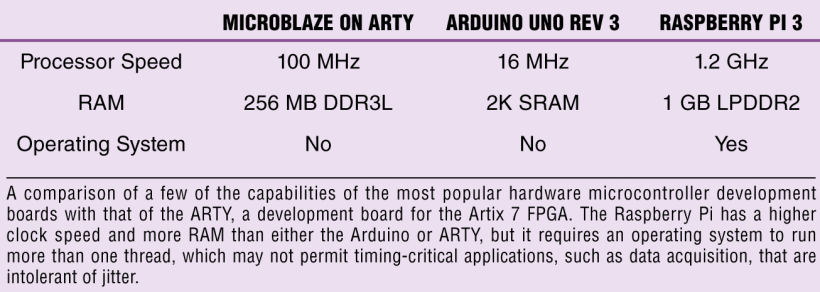
\includegraphics[scale=0.35]{romeo.t1-2733341-large (1).png}
\end{center}
  \caption{Hardcore vs Softcore \cite{3}}
  \label{fig3}
\end{figure}

\begin{itemize}
    \item \textbf{Performance Trade-offs:} The \textbf{MicroBlaze on ARTY}, representing softcore processors, offers a middle-ground performance with its 100 MHz processing speed, striking a balance between the \textbf{Arduino Uno's} lower 16 MHz and the \textbf{Raspberry Pi 3's} superior 1.2 GHz.
    
    \item \textbf{Memory Considerations:} Memory capacity often dictates the kind of applications a platform can support. \textbf{Arduino Uno's} minimal 2K SRAM is suitable for lightweight tasks, while the \textbf{Raspberry Pi 3}, with its 1 GB LPDDR2, is equipped to handle more memory-intensive applications. The \textbf{MicroBlaze on ARTY} finds a median with 256 MB DDR3L, offering versatility.
    
    \item \textbf{System Complexity:} The requirement of an operating system, as seen with the \textbf{Raspberry Pi 3}, introduces potential complexities, especially for real-time applications. In contrast, both the \textbf{MicroBlaze on ARTY} and \textbf{Arduino Uno's} design simplify real-time application deployment due to the lack of a mandatory OS.
    
    \item \textbf{Conclusion:} Softcore and hardcore processors cater to different niches, with the former often being more adaptable and the latter generally optimized for specific tasks. The data suggests a clear gradient from the simpler, dedicated functionality of the \textbf{Arduino Uno} to the more versatile yet complex \textbf{Raspberry Pi 3}, with the \textbf{MicroBlaze on ARTY} providing a harmonized middle ground.

The difference in performance and RAM between hardcore and softcore systems is significant, underscoring a well-recognised principle: hardcore systems typically outperform their softcore counterparts. However, it's crucial to understand that softcores are not often intended as final solutions; rather, they are instrumental in developing these solutions. For instance, a softcore can be utilized to prototype the desired functionality of a Raspberry Pi 3, leading to the Raspberry Pi 3 as the ultimate outcome of the process. The greatest advantage of softcores lies in their rapid prototyping capabilities and configurability, a fact that is essential to acknowledge in the realm of system design.
\end{itemize}
\newpage
\subsection{\textbf{Hardcore vs Softcore: Comparative Analysis 2}}
\begin{itemize}
\item \textbf{Design Flexibility:} Softcore processors, like the MicroBlaze implemented on the Virtex-II Pro FPGA, offer significant design flexibility. This is demonstrated by the block diagrams (Fig. 4 and Fig. 5) which show a customizable integration of various peripherals such as UART, interrupt controllers, timers, and GPIO. In contrast, hardcore processors are often fixed in their architecture and integration capabilities \cite{1}.

\item \textbf{Integration with FPGAs:} The block diagrams highlight how softcore processors are embedded within an FPGA fabric, such as the Xilinx ML310 development platform, allowing for a tailored system that fits specific application needs. This contrasts with hardcore processors, which are typically standalone and do not offer the same level of on-chip integration with an FPGA \cite{1}.

\item \textbf{Performance Considerations:} While the PowerPC405 runs at 100 MHz, it is a representative example of a hardcore processor that may offer more predictable performance due to its fixed architecture. Softcores like MicroBlaze can be configured to run at similar clock speeds but may have variable performance depending on the FPGA implementation and other design choices \cite{1}.

\item \textbf{Complexity of Implementation:} Implementing a softcore processor requires an understanding of FPGA programming and design, as it involves configuring the FPGA logic to emulate processor functionality. This complexity is not present with hardcore processors, which can be used out-of-the-box without the need for such configuration \cite{1}.

\item \textbf{Use Case Scenarios:} The work of \cite{1} details the implementation architecture based on the Microblaze softcore, suggesting its suitability for complex, multi-peripheral integrations within an FPGA. This is ideal for research, prototyping, or custom applications. Hardcore processors, meanwhile, are likely more suited to standard applications where the design requirements are known and less variable.
\end{itemize}
\begin{figure}[ht]
  \centering
  % Image 1
  \begin{minipage}[b]{0.45\linewidth}
    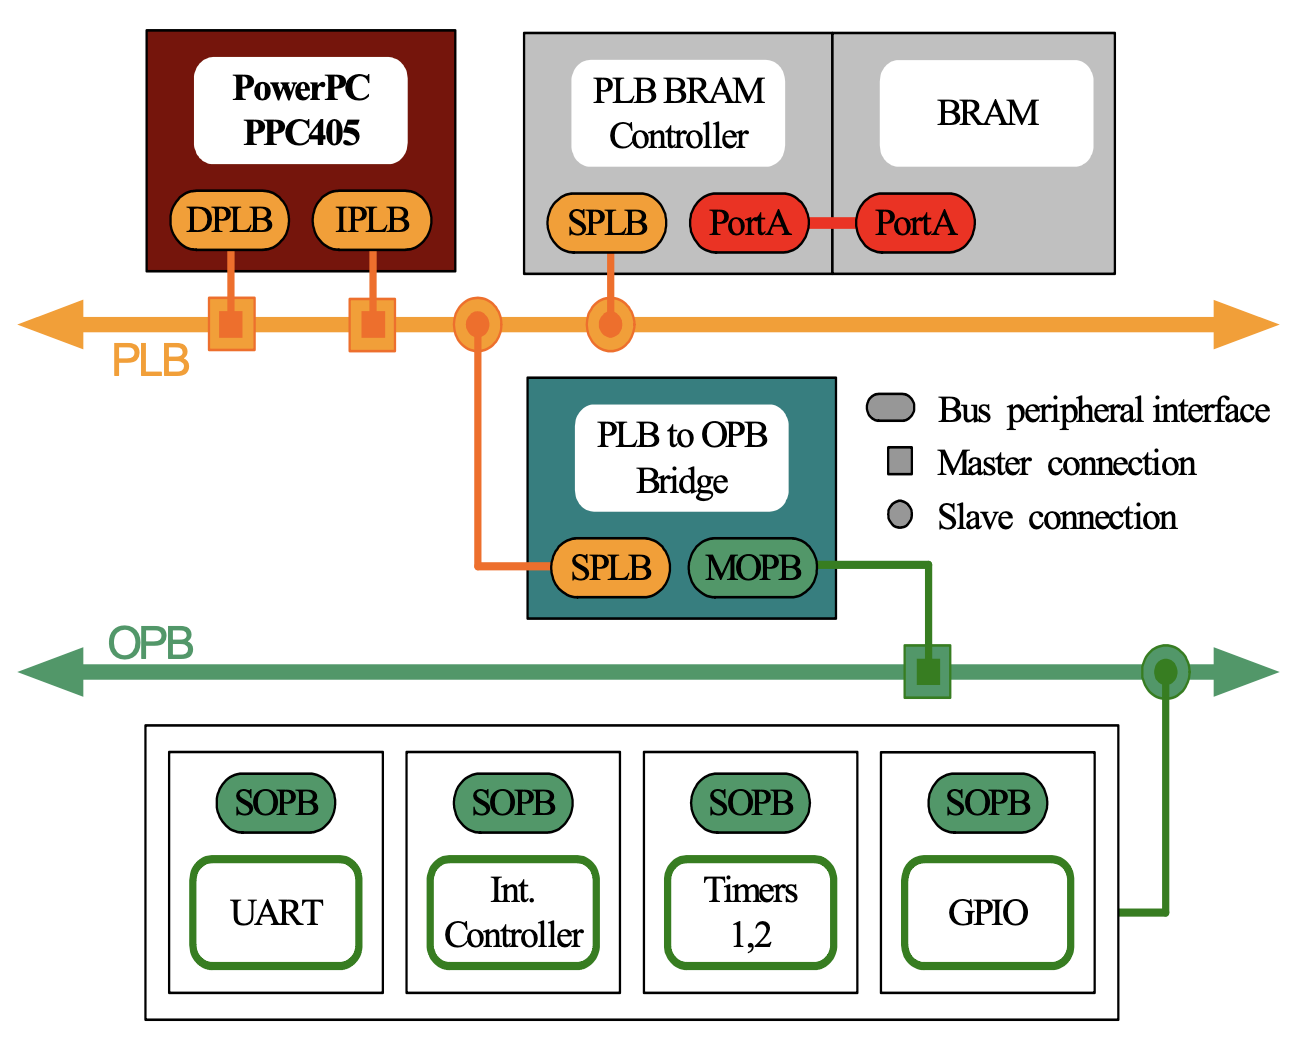
\includegraphics[width=\linewidth]{Screenshot 2023-11-08 at 19.59.01.png}
    \caption{PPC 405 BASED DESIGN}
    \label{fig:image1}
  \end{minipage}
  \hfill % this will insert a space between the two images
  % Image 2
  \begin{minipage}[b]{0.45\linewidth}
    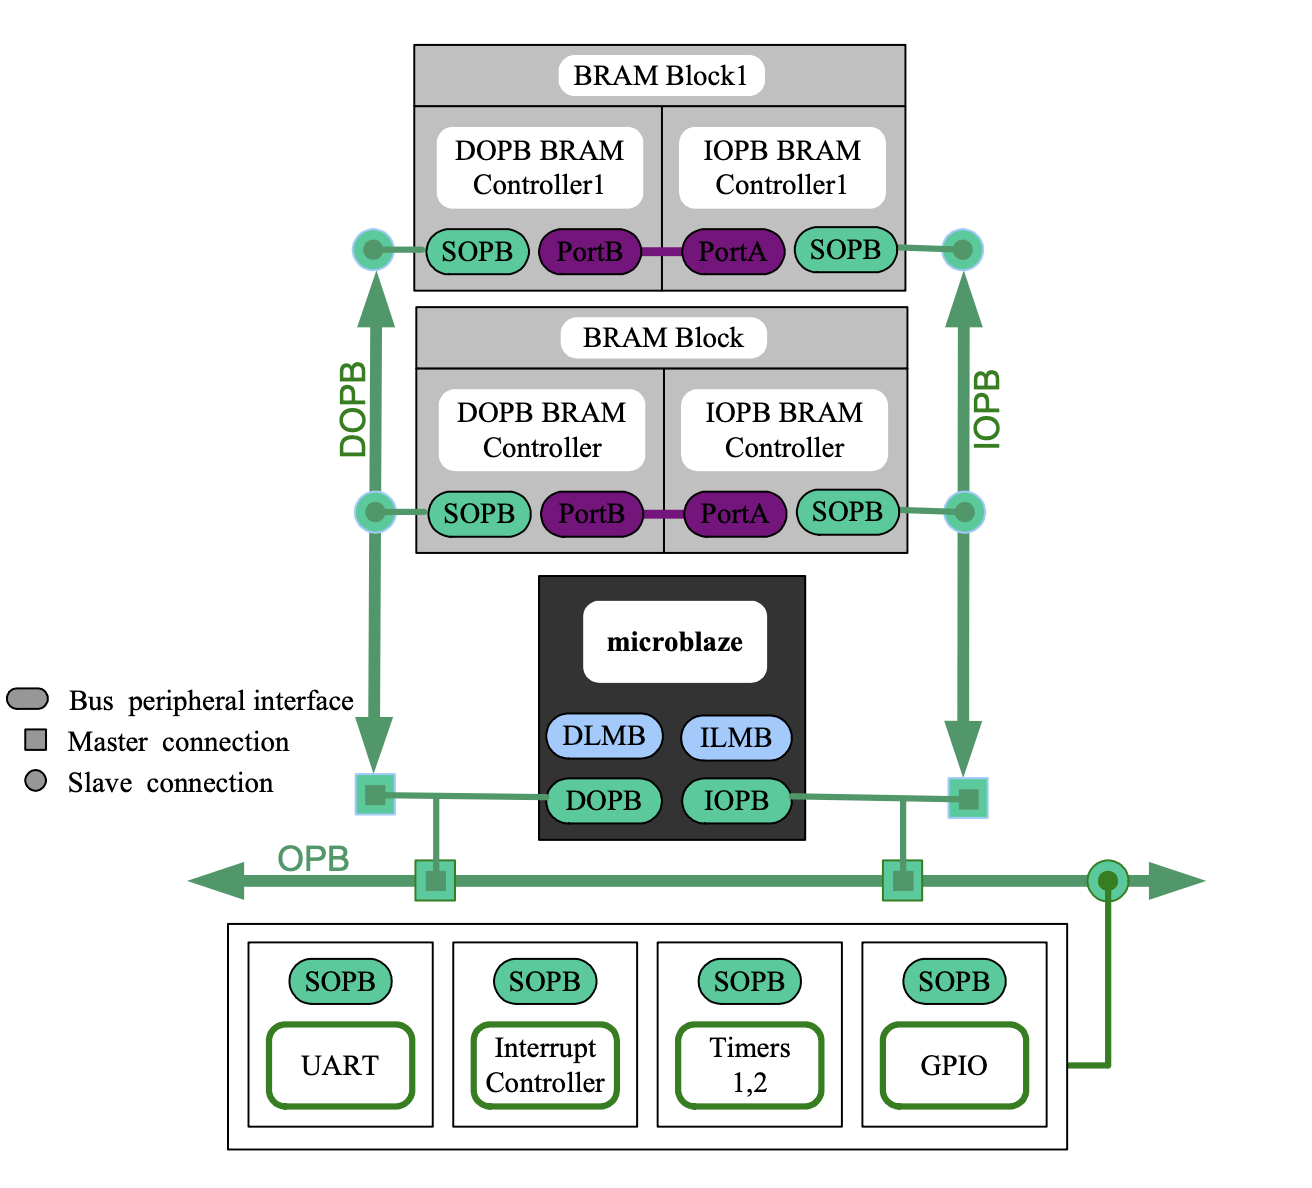
\includegraphics[width=\linewidth]{Screenshot 2023-11-08 at 19.59.27.png}
    \caption{Microblaze Based Design}
    \label{fig:image2}
  \end{minipage}
\end{figure}


\section{RISC-V}
The evolution of process architecture has been dominated in good parts by Complex Instruction Set Computing (CISC). While CISC architecture has been a revolutionary development in bridging the gap between high-level language and computer architecture in its time, it now encounters challenges such as increased complexity, power consumption, and limitations in scalability.
As technology progresses to the era of Industry 4.0, which is characterized by the integration of smart technologies and the demands of applications like the Internet of Things (IOT) and machine learning, these challenges have become more obvious and lead to some inefficiencies. This calls for a shift toward a more efficient and customizable architecture. In response to these evolving requirements, reduced instruction set computing five (RISC-V) becomes an interesting and compelling alternative. RISC-V architecture, known for its simplicity, modularity, and performance advantages, addresses most of the shortcomings of CISC, the open-source and customizable nature of the RISC-V ISA stands out. RISC-V ISA embodies all the attributes of RISC architecture and also introduces an open standard that allows for collaboration and innovation. This section explores the drawbacks of CISC in comparison to the innovative realm of RISC and tentatively explores RISC-V in the area of VLSI design. By delving into some specifics of RISC architecture, we aim to shed light on its potential to not only meet the demands of modern computing but also pave the way for a new era of open and collaborative processor design \cite{15}.
\subsection{Instruction Set Architecture (ISA)}
An Instruction Set Architecture (ISA) is a standard that outlines how a hardware processor should function and interact with an assembly language. Understanding what an ISA is helps to comprehend the significance of RISC-V. An ISA contains the necessary information for creating a processor capable of running machine code correctly. Its key aspects include elements such as instructions, registers, memory access, arithmetic, and data buses. The ISA dictates the processor's functionality, leaving the specifics of hardware design to the discretion of the designer. RISC-V is a prominent example of an ISA. Developed collaboratively by the University of California and companies like AMD, Google, Microsoft, and IBM, RISC-V presents a competitive alternative to proprietary and restricted commercial ISAs, such as those from Intel, AMD, and ARM \cite{13}.
\subsection{Key feature of RISC-V}
\begin{itemize}
\item \textbf{Open source}: 
One of the most significant advantages of RISC-V is its open-source nature, which not only spurs collaboration and innovation but also eliminates the financial and legal barriers typically associated with proprietary systems. This aspect makes it particularly appealing for educational institutions to incorporate into curriculum and research, startups to experiment with custom chip designs, and large-scale enterprises to consider cost-effective infrastructure upgrades. RISC-V's open-source model promotes its use everywhere, from schools to advanced tech industries.
\item \textbf{Extensibility}:
The fundamental specification of RISC-V, along with its standard extensions, can be immediately applied to novel chip designs, easing the development of basic computers with peripherals. Furthermore, the extensibility of this system is one of its special strengths. Its basic specification permits the integration of proprietary, user-defined extensions, allowing for customisation and adaption to particular requirements \cite{15}.


\end{itemize}
\subsection{Importance in Soft processors}
\begin{itemize}
   \item \textbf{Performance Over Complexity in Soft Core Design}: The RISC (Reduced Instruction Set Computer) architecture, with its emphasis on performance optimization over complexity, presents a significant advantage for softcore processor design. Soft cores, which are often employed in the prototyping of specific designs, benefit from the RISC philosophy because it leads to simpler, more predictable, and more efficient execution of instructions. This is particularly advantageous in a prototyping environment where design iterations need to be fast and cost-effective. The complexity of CISC might introduce excess resource consumption on the FPGA and potential difficulties in optimizing the processor’s performance due to the more intricate control logic required \cite{5}.
   
     \item \textbf{Efficient Use of Registers}: RISC's emphasis on using registers effectively is beneficial for softcore processors as it utilizes the fastest accessible memory for operations. 
    \item \textbf{Load/Store Architecture}: RISC's load/store approach simplifies the memory access model, which can benefit softcore processors by making them more efficient \cite{5}.

    \item \textbf{Modular Design}: The modular design of RISC enhances softcore development by allowing for efficient allocation of resource use within the FPGA. This is crucial for softcore design as it simplifies customization, making it superior to hardcores, which will consume time and resources to customise \cite{5}.
     \item \textbf{Pipelining}: One key component in RISC architecture's adaptation to softcore design is its ability to execute pipelining more effectively than CISC architecture. Increased system efficiency is achieved through pipelining, which is the simultaneous execution of several instructions in parallel. Softcores can get increased clock rates by decreasing the execution route and optimising the use of resources. This implies that we can adjust performance to meet the demands of a certain application \cite{5}.
     \item \textbf{Open source}: One of the most important reasons why RISC-V is being integrated into modern designs is its open-source nature.
     
\end{itemize}


\section{Soft RISC-V CORES}
\subsection{Introduction to Soft RISC-V Processors}
Having discussed what a soft processor is, along with what RISC-V architecture is, the focus now is going to be on a particular type of soft processor, which is the risc-v cores. Due to the rise of the RISC-V, which is aided especially by its open source nature and also the free customization of its ISA and micro-architecture, a lot of risc-v softcore implementation exists today \cite{6}.


\subsection{Existing soft RISC-V cores}
\begin{itemize} 

\item\textbf{PicoRV32}

The PicoRV32 core stands out as a compact and efficient RISC-V implementation that is particularly suited for auxiliary processing in FPGA and ASIC designs. Its design is focused on the RV32IMC instruction set, though it is configurable for the RV32E, RV32I, RV32IC, RV32IM, or RV32IMC core options, providing flexibility for a variety of applications. This versatility is further enhanced by the ability to add custom instructions and support for interrupt handling \cite{8}.

Featuring a small footprint, typically requiring between 750 to 2000 LUTs in 7-Series Xilinx architecture, the PicoRV32 offers a high maximum frequency of operation (250-450 MHz on 7-Series Xilinx FPGAs). It's designed with a selectable native memory interface or AXI4-Lite master, optional IRQ support, and a co-processor interface, enabling it to be integrated seamlessly into diverse system designs \cite{9}.

The state machine of the PicoRV32, as illustrated in the figure \ref{fig:4}, underscores its efficient processing pipeline. This pipeline is optimized to handle a typical ALU instruction flow, PCPI flow, and stalls due to instruction dependencies, ensuring that the core maintains high performance while minimizing resource usage \cite{8}. 
In essence, the PicoRV32 core exemplifies the minimalist design philosophy within the RISC-V ecosystem, demonstrating that high performance and energy efficiency can be achieved without an extensive transistor budget \cite{8}.
\begin{figure}[ht]
\begin{center}
  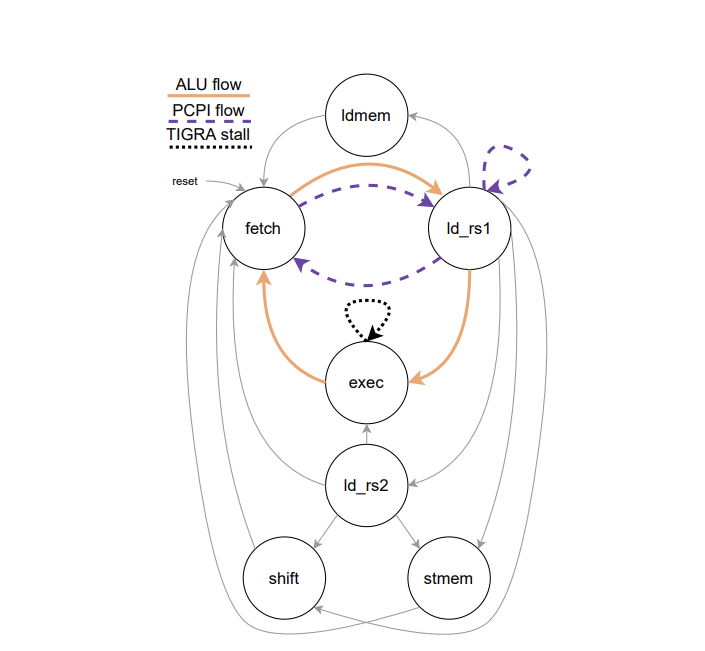
\includegraphics[scale=0.28]{Screenshot 2023-11-17 at 18.53.50 (1).png}
\end{center}
  \caption{PicoRV32}
  \label{fig:4}
\end{figure}


\item\textbf{NeoRV32}
In the landscape of RISC-V soft cores, the NeoRV32 emerges as a versatile and comprehensive open-source processor system, designed to facilitate the adoption of the RISC-V ISA in a variety of applications. This synthesizable soft core embodies the RISC-V RV32I instruction set, providing a robust foundation for both educational endeavours and practical implementations. The NeoRV32's architecture is characterized by its integration of a rich set of peripherals, a pre-configured bootloader, and a runtime environment, which collectively streamline the development process for FPGA platforms. The NeoRV32's adaptability is further enhanced by its configurable instruction set, which includes support for the RV32IM instruction set extension, thereby enriching its computational prowess. This extension expands the core's capability to handle integer multiplications and divisions, an essential feature for arithmetic-intensive tasks. As a testament to the RISC-V ecosystem's flexibility and open accessibility, the NeoRV32 stands as a prime example of how soft cores can democratize and accelerate processor design and deployment in the modern era of computing \cite{10}.






    \item \textbf{SiFive Performance Family (P650/670 series)}
    
This processor focuses on performance and efficiency; it was designed to cater to a wide range of applications. It operates under a 13-stage, 4-issue, out-of-order pipeline architecture. This advanced architecture allows increased instruction throughput and efficient high-level handling of parallelism, which significantly increases its computational performance. The most ideal use case for this processor is complex computer-intensive tasks such as machine learning. This processor also has full support for RVA22 RISC-V profile, vector 1.0, and vector crypto, which enables it to be compatible with a wide range of applications like graphics processing and encryption. The company claims it has a benchmark score of over 12SpecINT2k6 GHZ, which indicates exceptional interger processing performance and all-round performance.
In summary, the P650/670 series' capabilities make it highly suitable for applications that demand high processing power, parallelism, and efficient handling of complex computations, including applications in AI, data centres, and high-performance embedded systems. Its compatibility with the RISC-V ISA also means it benefits from the open, modular architecture of RISC-V, offering potential for further customization and optimization in FPGA and ASIC implementations \cite{12}.


    \item \textbf{SiFive Automotive Family (E6-A series)}
This family is tailored for the automotive sector, particularly for 32-bit real-time applications. The various variants (E6-AB, E6-AD, E6-AS) are designed to meet different Automotive Safety Integrity Levels (ASIL), making them suitable for a range of automotive applications from system control to advanced driver-assistance systems (ADAS). The single-issue, in-order 8-stage Harvard Pipeline ensures efficient processing, crucial for real-time automotive applications. The support for 32-bit physical addressing and a variety of floating-point precisions makes these processors flexible for different automotive computing needs. Their functional safety up to ASIL D is essential for meeting the rigorous safety standards required in the automotive industry \cite{12}.
    
  
    \item \textbf{SiFive Intelligence Family (X280)}
These processors are specifically optimized for artificial intelligence and machine-learning edge computing. X280 is a multicore-capable RISC-V processor with vector extensions and SiFive Intelligence Extensions. The 512-bit vector register length and the 8-stage dual-issue in-order pipeline provide significant computational power for AI/ML tasks, including inferencing and data processing. This processor is ideal for applications that require high-throughput, single-thread performance under power constraints, like augmented reality (AR), virtual reality (VR), and sensor hubs. Being Linux capable and supporting configurations up to 8 cores, the X280 is versatile for various high-performance applications, ensuring it can handle demanding AI and ML workloads effectively \cite{12}.


 \item \textbf{ SiFive Freedom E310 (FE310) }
 This is another notable RISC-V processor. It is designed for a wide range of applications and features SiFive’s E31 RISC-V Core, a high-performance 32-bit RV32IMAC core capable of running at over 320 MHz, positioning it among the fastest microcontrollers on the market. Key features of the FE310 include a 16KB L1 Instruction Cache and a 16KB Data SRAM Scratchpad, hardware support for multiply/divide operations, a debug module, and one-time programmable non-volatile memory (OTP). It also offers flexible clock generation with on-chip oscillators and PLLs. The FE310 supports a variety of peripherals, including UARTs, QSPI, PWMs, and timers, and it incorporates multiple power domains and a low-power standby mode, making it highly versatile for different applications \cite{11}.


\end{itemize}

\subsection{Comparative Analysis of Soft RISC-V Cores}
Each softcore is designed according to certain requirements and applications; this is seen in the SiFive Intelligence family, which is designed specifically for AI and ML applications. Similarly,  with the automotive family E6-a Series, tailored to the needs of automotive devices, the PicoRV32 cannot perform these intensive tasks and is best suited for space-constrained applications and educational purposes. The NeoRV32 is another general-purpose core not suited to the high demand of intensive computing. The SiFive Performance Family (P650/670 series) and the Freedom E310 offer high processing power, but the E310, being a microcontroller, might not match the P650/670 series in handling complex, parallel tasks. Overall, while some cores could theoretically replace others in general applications, their specialised features often make them uniquely suited to particular domains. 

\section{Hard RISC-V cores}
\textbf{Esperanto’s ET-SoC-1 Chip:} 

This chip is the highest-performing RISC-V chip on the market. It comprises over a thousand RISC-V processors on a single TSMC 7nm chip. It includes 1088 energy-efficient ET-Minion 64-bit RISC-V in-order cores, each with a vector/tensor unit, and 4 high-performance ET-Maxion 64-bit RISC-V out-of-order cores. Additionally, it has more than 160 million bytes of on-chip SRAM. Its additional features include interfaces for large external memory with low-power LPDDR4x DRAM and eMMC FLASH, along with PCIe x8 Gen4 and other common I/O interfaces, among others. The ET system on chip is a general-purpose parallel processing system that is better utilized when there is an intensive workload. It is recommended for use in demanding applications like machine learning. The entire design of the ET-SoC-1 is geared towards achieving high levels of energy efficiency, making it a prime example of the capabilities and potential of RISC-V soft cores in modern computing applications, especially in AI and machine learning. Most machine learning-specific chips use one giant hot chip that consumes high power, making it energy inefficient while also offering limited parallelism. However, the Esperanto ET SoC-1 uses multiple low-power chips that still fit within a power budget and also offer full parallelism, with thousands of cores always available. Esperanto also supports C++, PyTorch, and common ML frameworks \cite{7}. 



\section{Implementation Examples}
The RISC V ISA  has gained prominence in a range of fields, one of which is the Internet of Things. This is due to its robust security features and open-source nature. This enables it to compete with already established products like ARM. The work of \cite{14} details the design of a lightweight open-source implementation of a RISC-V processor, which is tailored to be implemented on an FPGA \cite{13}.


The primary goal is to craft a design that's both lightweight and accessible for beginners, suitable for deployment on small FPGAs. This strategy is intended for educational use, enabling students to gain insights from a streamlined yet operational RISC-V processor. For this design, complex conventions and components typically present in modern processors were omitted. Features like pipelining weren't incorporated, and a straightforward Harvard architecture was utilized instead. Nevertheless, this system is designed for potential upgrades in almost every aspect, although it involves the use of SystemVerilog \cite{13}.

\subsection{Results }
\paragraph{Instruction Execution:}
After successful design and testing of the CPU in System Verilog, some test runs were conducted.

In Figure \ref{exe}, we see an example of a Fibonacci sequence instruction for our processor. Each instruction is executed within one cycle, demonstrating the processor's ability to handle iterative computations \cite{13}.

\begin{figure}[ht]
\begin{center}
  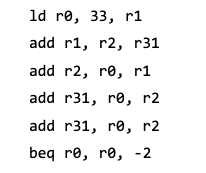
\includegraphics[scale=0.65]{Screenshot 2023-11-23 at 00.05.19 (1).png}
\end{center}
  \caption{Fibonacci Sequence\cite{13}}
  \label{exe}
\end{figure}
\paragraph{FPGA Utilization Metrics:}
The work showcases commendable FPGA resource efficiency. Figure \ref{eff} in the original document indicates minimal utilization of the FPGA's resources: only \textbf{1.55\%} of look-up tables and \textbf{0.55\%} of flip-flops, which suggests an economical design suitable for educational platforms or low-resource applications \cite{13}.

\begin{figure}[ht]
\begin{center}
  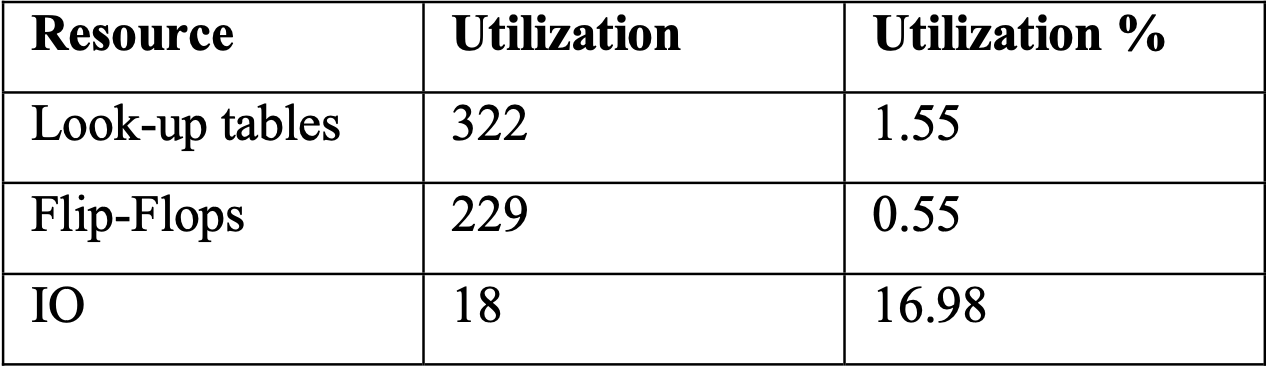
\includegraphics[scale=0.15]{Screenshot 2023-11-23 at 00.20.17 (1).png}
\end{center}
  \caption{Utilization Metrics\cite{13}}
  \label{eff}
\end{figure}



\paragraph{Benchmarks:}
The authors benchmarked their processors using the Dhrystone test, a widely-recognized standard for evaluating processor performance, especially in integer arithmetic operations. Their results, depicted in Figure \ref{ben}, showed that the softcore processor achieved performance on par with well-known architectures such as the ARM Cortex-A9 when normalized for clock speed \cite{13}.
\begin{figure}[ht]
\begin{center}
  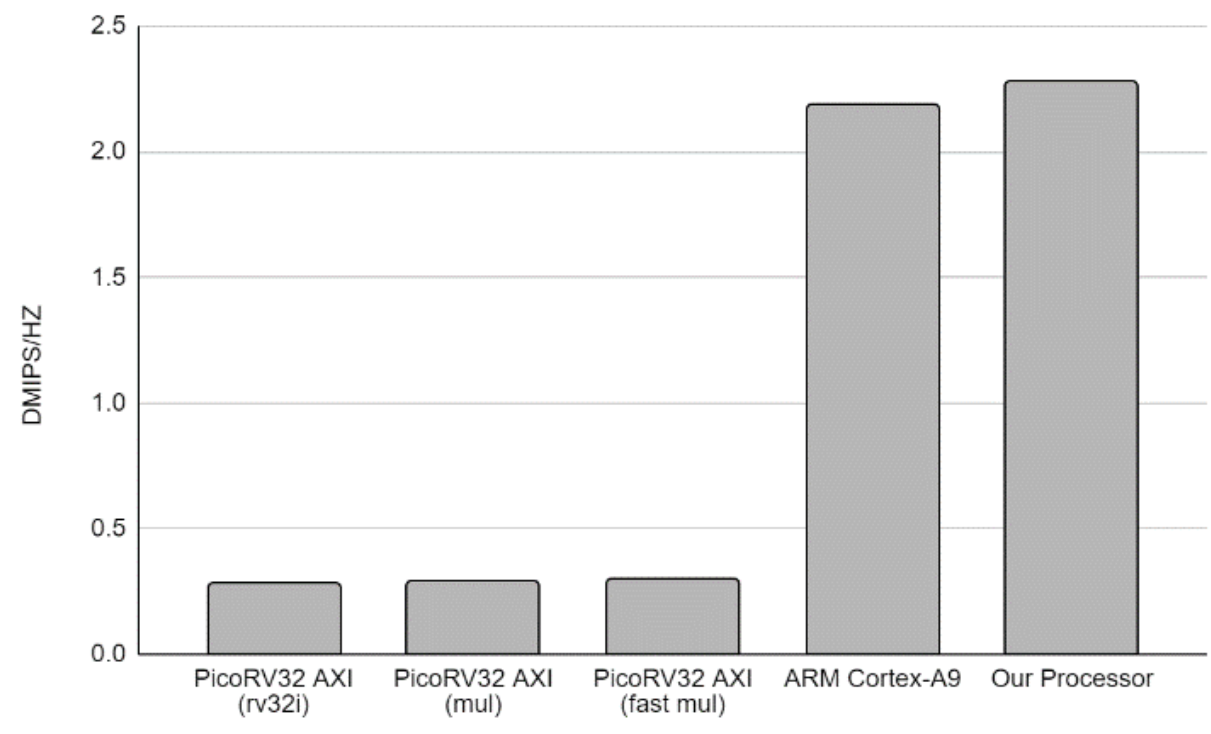
\includegraphics[scale=0.15]{Screenshot 2023-11-23 at 00.20.48 (1).png}
\end{center}
  \caption{Benchmark\cite{13}}
  \label{ben}
\end{figure}

This benchmarking result using the Dhrystone test (a renowned standard for processor performance evaluation) reveals that when the RISC-V processor is normalised for clock speed, the RISC-V softcore processor implemented in this example archives similar performance levels to an established architecture like the ARM Cortex-A9, despite being a simplistic form without advanced features like pipelining. This parity in performance underscores RISC-V efficiency and its potential as an option in the realm of high-performance computing.


\newpage
\section{ Challenges and Future Directions}
\subsection{Challenges of Soft-Core Processors:}
\begin{enumerate}
    \item \textbf{Vulnerability to effects of (SEUs):} Single Event Upsets (SEUs) are changes in the state of a digital logic circuit brought about by external factors such as radiation. These events can cause a bit of a flip from 0 to 1. In hardcore processors, the impact of SEUs is significantly lower; however, this poses a greater risk in softcore and especially in space applications. The reason for this is that softcore is implemented in programmable logic, making it more susceptible to SEUs. Engineers must consider these factors when developing a system and choosing between hardcore and softcore as their central processor \cite{14}.
    \item \textbf{Performance:} As shown in the comparison section between hardcore and softcore processors previously, a softcore processor will most likely trail behind hardcore processors in terms of performance. This is mostly because other solutions, such as ASICS, are optimised for specific tasks as customer-designed hardware.
    \item \textbf{Clock Speeds:}  The maximum achievable clock speed for a softcore processor is generally lower than that of a dedicated hardware processor. This is due to the overhead introduced by the FPGA's programmable logic.
      \item \textbf{Scalability:} Scaling a softcore processor for more complex applications can be challenging due to the fixed resources available on the FPGA.
\end{enumerate}

\subsection{Future Direction:} Looking ahead, research should pivot towards addressing the challenges detailed in this paper, most especially the SEUs and soft errors, with a specific focus on RISC-V cores. Robust error correction and mitigation techniques should be developed in order to improve the reliability of softcore processors in various applications. Also, the computational abilities should be enhanced to a level that they can compete with clock speeds and performance produced by hardcore processors. The advantages of rapid prototyping, combined with increased scalability, can prove immense in the industry of IC design. This can cut a lot of costs when done on a large scale. An intriguing avenue for exploration is the integration of soft IP cores in emerging technologies such as quantum computing and AI, which could unveil new applications and breakthroughs in this field.
\newpage


\section{Conclusion}
With an emphasis on RISC-V processors, this study concludes by shedding light on the possibilities and difficulties of soft IP-cores in the field of IC design. Our investigation shows that soft IP-cores are a valued asset in today's technological world because of their adaptability and customizability. Because it is open-source, the RISC-V architecture stands out as a major force in encouraging creativity and adaptability in processor design. We are aware of the difficulties softcore processors face, too, including scalability problems, performance limitations, and vulnerability to SEUs. For soft IP-core technology to be widely adopted and advanced, several obstacles must be overcome.  Research efforts should be focused on improving the capabilities of soft IP-cores to make sure they stay essential in this rapidly developing industry.


\begin{thebibliography}{1}


\bibitem{1}
A. K. B. Salem, S. B. Othman, and S. B. Saoud, "Hard and soft-core implementation of embedded control application using RTOS," in \emph{2008 IEEE International Symposium on Industrial Electronics}, 2008, pp. 1896-1901.

\bibitem{2}
J. B. Nade and R. V. Sarwadnya, "The soft core processors: A review," \emph{International Journal of Innovative Research in Electrical, Electronics, Instrumentation and Control Engineering}, vol. 3, no. 12, pp. 197–203, 2015.

\bibitem{3}
D. Romeo, J. LaMagna, I. Hogan, and J. C. Squire, "An Introduction to Soft-Core Processors and a Biomedical Application," \emph{IEEE Potentials}, vol. 37, no. 2, pp. 13-18, 2018.

\bibitem{4}
M. Zaheer and A. M. Khan, "Development of Softcore Processor," \emph{International Journal of Research in Engineering and Technology (IJRET)}, vol. 4.

\bibitem{5}
M. Katevenis, "Risc Architectures," in \emph{$\Sigma$$\tau$o Parallel and Distributed Computing}, pp. 595-619.

\bibitem{6}
J.-M. Gorius, S. Rokicki, and S. Derrien, "Design Exploration of RISC-V Soft-Cores through Speculative High-Level Synthesis," in \emph{2022 International Conference on Field-Programmable Technology (ICFPT)}, 2022, pp. 1-6.

\bibitem{7}
D. Ditzel et al., "Accelerating ML Recommendation with over a Thousand RISC-V/Tensor Processors on Esperanto’s ET-SoC-1 Chip," in \emph{2021 IEEE Hot Chips 33 Symposium (HCS)}, 2021, pp. 1-23.

\bibitem{8}
D. W. Todd, "Tightly coupling the PicoRV32 RISC-V processor with custom logic accelerators via a generic interface," Ph.D. dissertation, Clemson University, 2021.

\bibitem{9}
YosysHQ, "PicoRV32 - A Size-Optimized RISC-V CPU," 2023. [Online]. Available:{https://github.com/YosysHQ/picorv32}

\bibitem{10}
S. Nolting, "NeoRV32: An Open-Source RISC-V Processor," 2023. [Online]. Available: {https://github.com/stnolting/neorv32}

\bibitem{11}
"Freedom E310," SiFive. [Online]. Available: \url{https://d2pn104n81t9m2.cloudfront.net/products/freedom-e310}

\bibitem{12}
SiFive, "Sifive Risc-V Core IP," 2023. [Online]. Available: \url{https://www.sifive.com/risc-v-core-ip}

\bibitem{13}
L. Poli, S. Saha, X. Zhai, and K. D. Mcdonald-Maier, "Design and Implementation of a RISC V Processor on FPGA," in \emph{2021 17th International Conference on Mobility, Sensing and Networking (MSN)}, 2021, pp. 161-166.

\bibitem{14}
N. H. Rollins and M. J. Wirthlin, "Reliability of a Softcore Processor in a Commercial SRAM-Based FPGA," in \emph{Proceedings of the ACM/SIGDA International Symposium on Field Programmable Gate Arrays}, 2012, pp. 171–174.
\bibitem{15}
Efinix, Inc., "RISC-V and FPGAs," Efinix, Inc. [Online]. Available: https://www.efinixinc.com/blog/riscv-and-fpgas.html. [Accessed: Dec. 17, 2023].
\end{thebibliography}

% that's all folks
\end{document}


